%%%%%%%%%%%%%%%%%%%%%%%%%%%%%%%%%%%%%%%%%%%%%%%%%%%%%%%%%%%%%%%%%%%%
% Medical Data and imaging
%%%%%%%%%%%%%%%%%%%%%%%%%%%%%%%%%%%%%%%%%%%%%%%%%%%%%%%%%%%%%%%%%%%%
%!TeX spellcheck = en-GB
\chapter{Medical Data and imaging}
    \label{Medical Data and imaging}
\section{DICOM Format}
\begin{wrapfigure}{r}{0.3\textwidth}
    \vspace{-10pt}
    \centering
    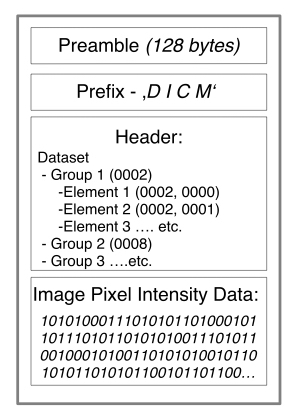
\includegraphics[width=0.28\textwidth]{figures/dicom.jpeg}
    \caption{structure of a DICOM file }
        \label{figure 2.1}
    \vspace{-15pt}
\end{wrapfigure}
DICOM  stands for Digital Imaging and Communications in Medicin. It provides standardized file format for medical images. Each DICOM file is made up of a header, holding meta data, and a body which contains the image. The meta data consists of a standardized series of tags which can be arranged in functional groups like "0010" patient information or "0008" study information.
DICOM images that are used for research or teaching are typically anonymized to protect the patients data. There are special programms to remove the according parts from the header.
The DICOM standard has the advantage that it can store all data that would ever be necessary. Still, outside of a clinic it can lead to a few problems. DICOM files tend to be fairly large, as they usually contain quite a few high resolution images.
Since DICOM files are not recognized as image files by most operating systems, including windows, macOS and ubuntu, they can only be viewed with the help of third-party software.
Thats why most equipment manufacturers either include a dicom viewer when the images are exported to a CD or just convert them to a JPEG, GIF or TIFF.
\cite{varmaManagingDICOMImages2012}
 \cite{ElsevierEnhancedReader}

  \section{Image Aquisition}
 \label{Image Aquisition}
 There are many different types of medical imaging. Each method has their own purpose and often more than one type of image is required to make a correct diagnosis. The first most common and also foundation for all other type of imaging techniques being an X-ray scan. It is on of the fastest methods to check for a bone fracture or tooth decay. However,  an X-ray don't have a depth of field therefore only show one view through the patients body. Hence, sometimes an important detail can't be seen because it lies behind a less permeable material. PET Scans, CTs and MRI Scans give us the option to image the whole volume or a planar slice thorugh it. In the following I will give a quick summary on 2d, 3d, 4d and CINE imaging techniques and their datasets using the MRI scanning methodology as an example.

 \subsection{2d Slices}
    \label{2d Slice}
 In an MRI scanner a magnetic field is created, so that all protons in the patients body align themselfs with that field.
A 2d image is created by exciting a slice of tissue with a radio frequency (RF) impulse so that the protons in said tissue spin out of equilibrium. Two types of relaxation times can be measured. The longitudal relaxation, which is the time it takes for a proton to realign with the surrounding magnetic field. The transverse relaxation occurs when the spins dephase and therefore return to their Lamor frequency.
\cite{MagneticResonanceImaging}
\cite{vangeunsBasicPrinciplesMagnetic1999}
The thickness of the slices depend on the device used, but are normally between 2mm and 100mm.
\cite{lineyMRIRadiotherapyPlanning2019}
Modern machines are able to excite multiple slices of tissue, therefore making it possible to scan multiple slices at a time. This technique is called a 2D Multislice MRI.
\cite{johnson2DMultislice3D1999}
\cite{vangeunsBasicPrinciplesMagnetic1999}

  \subsection{3d Volumetric imaging}
  \label{3d Volumetric imaging}
  There are two main ways to get a 3d image. One of these being a reconstruction of the original volume thorugh a collection of 2d slices. This sounds very simple, but there are actually may things to consider. Firstly, scantimes can be quite long, as there needs to be a short pause inbetween scans. Pictures need to be taken in the exact same position to avoid artifacts. Furthermore there will always be a space inbetween two slices. With methods such as the distance field interpolation, we have tools to overcome this proplem to a certain extent, but it will never be as exact as the second method of 3d imaging.
  \cite{vangeunsBasicPrinciplesMagnetic1999}
  Here, a whole slab of the volume gets excited.


  \subsection{4d MRI}
  \label{4d MRI}
  4d MRI, also known as 4d flow MRI, is the process of generating multiple 3d images with an added fourth dimension: movement. More specifically, the movement of fluids like blood or cerebrospinal fluid.
  \cite{bunckMagneticResonance4D2012a}
  \cite{stankovic4DFlowImaging2014}

  \subsection{CINE MRI}
   \label{CINE MRI}
    The human body naturally moves at all times. Respiratory and cardiac motion, as well as digestion and muscle movements, cause the movement of surrounding tissues. For example, to get a clear image of a patients heart, they are asked to hold their breath since the inflation of the lungs causes the heart to move up and forward a bit. It has always been a challenge to capture movements in 3d medical images or get an image in a good position to see a certain feature. With CINE imaging, medical professionals are able to capture the body in motion and pick the best time frames for their issue. It also enables us to record the activity and functioning of an organ which can most of the time give a useful context to a still image.

   \paragraph{2d CINE MRI}
   Originally this was the only way to record a CINE MRI sequence. A 2d slice image is created at a high frequency at different positions in the region of interest (ROI).
   To monitor out of plane movement, a orthogonal CINE MRI can be made. This procedure takes a

  \paragraph{Volumetric CINE MRI}
  Volumetric CINE MRI (VC - MRI) is relatively new and still under development. It follows a similar principle as 2d CINE MRI, but instead of using 2d slices, a 3d volume is being recorded for the CINE sequence.
  The main advantage of this new technique is it's superiority in on-board target localization to the 2d CINE MRI and 4d MRI. The accuracy of this method is constantly improving.
  \cite{harrisVolumetricCineMagnetic2020}

\section{Image-guided therapy}
    \label{Image-guided therapy}
In image guided therapy, clinicians make use of all kinds of medical images such as MRT and CT, to help them plan, perform, monitor and control therapeutic procedures.
The used image data is aquired before, during or after the treatment and usually heavily rely on some sort of radiology.
\cite{helmbergerRadiologistsLeadingPosition2013}

\subsection{planning}
    \label{planning}
When planning an operation or radiation session, MRI is mainly used for gross tumor volume (GTV) and organs at risk (OAR) delineation.
\cite{lineyMRIRadiotherapyPlanning2019}

  \subsection{radiotherapy and LINAC}
    \label{radiotherapy and LINAC}
stereotactic radiosurgery (SRS)
